\chapter{Deseño de software}
O longo deste capítulo detállase a arquitectura do sistema a desenvolver. Mostrase primeiro a arquitectura xeral e a súa interacción con sistemas externos e posteriormente detallase máis polo miúdo a estrutura das distintas compoñentes do sistema e como cooperan entre elas para resolver cada un dos casos de uso definidos.

\section{Arquitectura do sistema}
Dende a definición dos obxectivos do proxecto se identifican dúas partes diferenciadas dentro do sistema a desenvolver. Por un lado a comunicación co servidor SOS, para a obtención das súas capacidades e dos datos de observacións, e por outro a visualización e explotación das observacións descargadas. Esta división trasladase directamente á estrutura da aplicación, que se amosa na figura \ref{fig:diaComponentes}, na que tamén se inclúen os compoñentes externos cos que se relacionan.

\begin{figure}[hbtp]
 \centering
 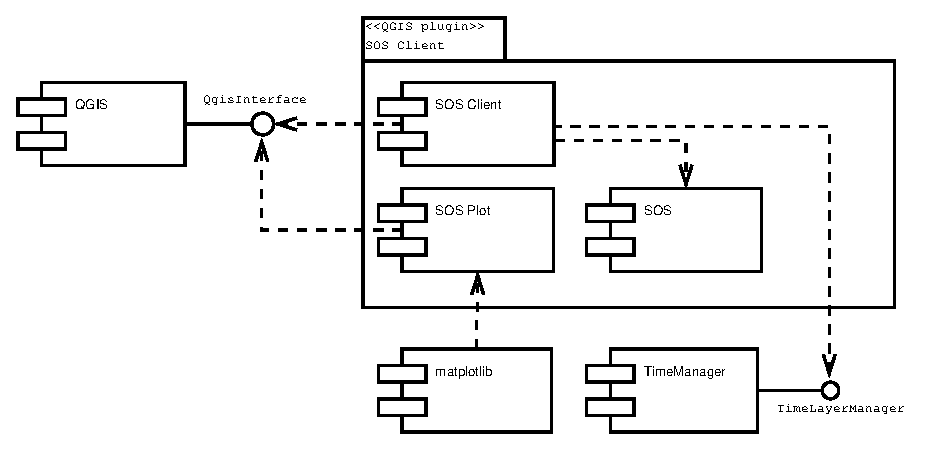
\includegraphics[width=0.5\textwidth]{images/componentes.eps}
 \caption{Diagrama de compoñentes}
 \label{fig:diaComponentes}
\end{figure}

A compoñente \textbf{SOS Client} é a responsable da comunicación co servidor SOS tanto a hora de xerar as peticións necesarias a partir da información proporcionada polo usuario e como para almacenar e interpretar as respostas do servizo.

A compoñente \textbf{SOS Plot} é a responsable de, a partir da capa vectorial xerada, visualizar as observacións segundo as preferencias indicadas polo usuario.

\subsection{Patrón de arquitectura}
O uso dun patrón de arquitectura axeitado para o sistema a desenvolver facilita os procesos de implementación e probas, ó proporcionar un esquema de organización estrutural dividindo o sistema en partes segundo a súa responsabilidade.

Os patróns de arquitectura máis amplamente utilizados no desenvolvemento de aplicacións son o MVC (\emph{Model-View-Controller}) e os seus derivados. O obxectivo principal destes patróns é separar o modelo de datos, a súa visualización e a lóxica de negocio facilitando de xeito moi significativo o mantemento e evolución das aplicacións.

Dadas as características concretas desde desenvolvemento optouse por unha simplificación do patrón MVC combinando a lóxica de negocio coas vistas, dando lugar a unha arquitectura denominada \emph{Model/View}\footnote{\url{http://doc.qt.io/qt-4.8/model-view-programming.html}}. Os motivos principais para levar a cabo esta simplificación son:
\begin{itemize}
\item A lóxica de negocio da aplicación e moi sinxela.
\item As librerías para o desenvolvemento das vistas veñen impostas pola aplicación na que se integrará o \emph{plugin}. As propias librerías están deseñadas para facilitar este patrón.
\end{itemize}

É importante destacar que aínda que se se incorpore a lóxica de negocio nas vistas, si que se mantén a separación entre a creación e configuración dos compoñentes gráficos do resto de lóxica da vista. A creación dos compoñentes gráficos faise a través dunha factoría que os xera directamente desde a súa definición XML.

Na figura \ref{fig:MVCvsMV} móstrase de xeito gráfico a diferencia entre o patrón MVC e o \emph{Model/View}. O \emph{Model/View}, amais da vista e o modelo, inclúe o concepto \emph{Delegate}, que representa a un mediador entre a vista e o modelo para facilitar a personalización de como se mostran e editan determinados datos.

\begin{figure}[hbtp]
 \centering
 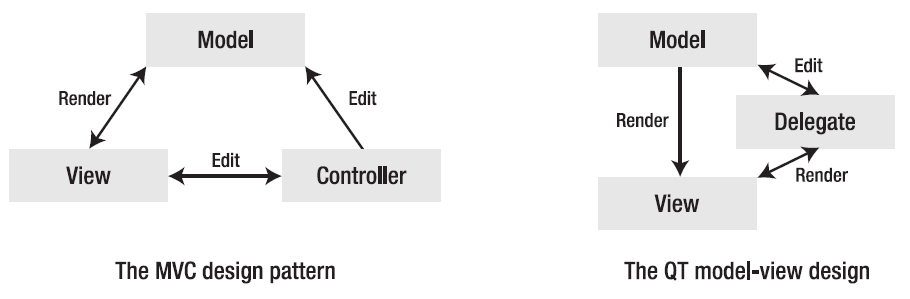
\includegraphics[width=\textwidth]{images/MVCvsMV.png}
 \caption{Diferencias entre MVC e Model/View}
 \label{fig:MVCvsMV}
\end{figure}

\section{Diagramas de clases}
A continuación descríbese máis en detalle cada unha das compoñentes do sistema a desenvolver, representando as clases máis relevantes de cada unha. Nos diagramas de clase so se mostran os atributos e métodos máis relevantes para entender o a función de cada unha delas.

No diagrama \ref{fig:diaClassSOSClient} represéntanse as clases correspondentes a compoñente SOS Client, separadas entre as que corresponde á vista e as que corresponden ó modelo. Represéntanse agrupadas sobre fondo escuro as clases encargadas do procesamento dos documentos XML proporcionados polo servizo SOS.

\begin{sidewaysfigure}
 \centering
 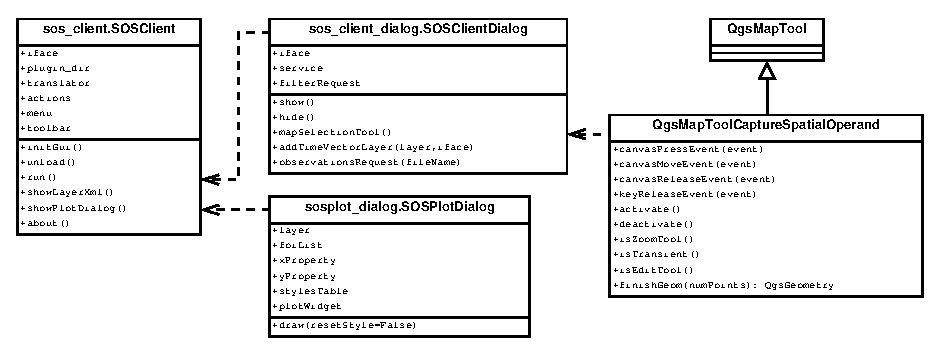
\includegraphics[width=\textwidth]{images/clases_sos_client.eps}
 \caption{Diagrama de clases da compoñente SOS Client}
 \label{fig:diaClassSOSClient}
\end{sidewaysfigure}

As clases máis relevantes da compoñente SOSClient son:
\begin{description}
\item[WidgetFactory:] Esta clase é unha factoría que crea a partir dos XML de definición da interface a clase cos compoñentes gráficos. A implementación real da vista farase en clases que herdarán da clase correspondente creada por esta factoría.
\item[SOSClientDialog:] É o formulario xeral de comunicación cos servidores SOS. Contén a lóxica de funcionamento da vista e as chamadas necesarias as clases que forman o modelo.
\item[SensorObservationService:] Esta clase representa o servizo SOS. Créase a partir do XML que define as capacidades do servizo e almacena toda a información necesaria para que a vista poda presentar o usuario as opcións correspondentes para xerar as consultas.
\item[ObservationsLayer:] Esta clase é a encargada de construír a capa vectorial para o QGIS, a partir da clase SOSProvider.
\item[SOSProvider:] Simula unha clase QgsVectorDataProvider\footnote{\url{http://qgis.org/api/classQgsVectorDataProvider.html}}. É pois a clase que fai de intermediaria entre a estrutura de datos real da información da capa e a estrutura manexada polo QGIS.
\item[XMLParserFactory:] Esta clase é unha factoría para crear as distintas clase para o procesamento dos XML. A partir da etiqueta XML atopada devolve a clase encargada de procesar o nodo.
\item[XMLParser:] Clase base para todas as clases de procesamento de XML.
\end{description}

No diagrama \ref{fig:diaClassSOSPlot} represéntanse as clases correspondentes a compoñente SOS Plot. Móstranse agrupadas todas as clases que cumpren co rol de \emph{Delegate}, e todas as demais forman parte da vista. Neste módulo o modelo non está representado no diagrama pois está composto por clases internas do QGIS (QgsVectorLayer) e de matplotlib (Line2D)

\begin{figure}
 \centering
 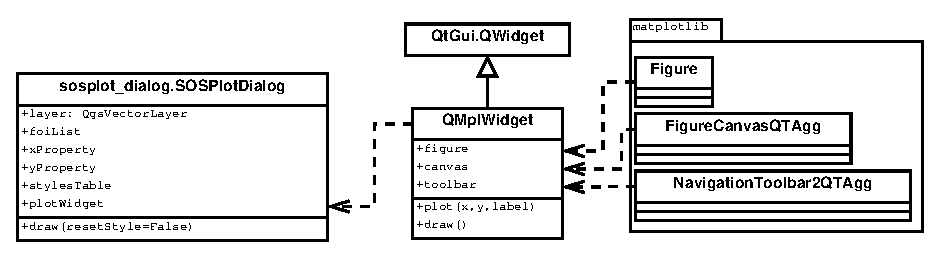
\includegraphics[width=\textwidth]{images/clases_sos_plot.eps}
 \caption{Diagrama de clases da compoñente SOS Plot}
 \label{fig:diaClassSOSPlot}
\end{figure}

As clases máis relevantes da compoñente SOSPlot son:
\begin{description}
\item[WidgetFactory:] E a mesma clase xa descrita no punto anterior, que actúa como factoría das compoñentes gráficas.
\item[SOSPlotDialog:] Es el formulario de visualización de gráficos. Filtra e transforma os datos da capa vectorial activa para visualizalos no QMplWidget e conecta os distintos \emph{Delegates} co modelo.
\item[QMplWidget:] Clase que amalgama os obxectos da librería matplotlib\footnote{\url{http://matplotlib.org/}} para a visualización de gráficos.
\end{description}

\section{Diagramas de secuencia}
Para describir o comportamento do sistema desde un punto de vista dinámico empréganse os diagramas de secuencia, nos que se describe a interacción entre as distintas compoñentes do sistema para cumprir cada caso de uso definido.

No diagrama \ref{fig:diaSeq1-2} inclúense os caso de uso \ref{uc:CU.01} e \ref{uc:CU.02}, xa que o \ref{uc:CU.02} estende ó \ref{uc:CU.01}, polo que é máis claro representalos xuntos.
\begin{figure}
 \centering
 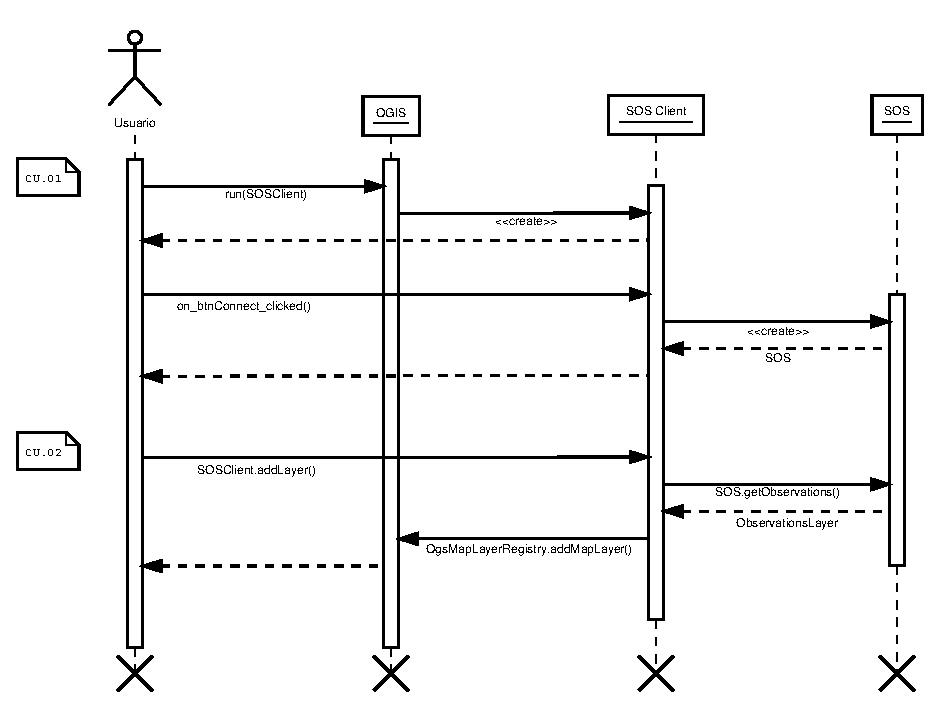
\includegraphics[width=\textwidth]{images/seq1-2.eps}
 \caption{Diagrama de secuencia para os casos de uso \ref{uc:CU.01} e \ref{uc:CU.02}}
 \label{fig:diaSeq1-2}
\end{figure}

O diagrama \ref{fig:diaSeq3} representa o comportamento para o caso de uso \ref{uc:CU.03}.
\begin{figure}
 \centering
 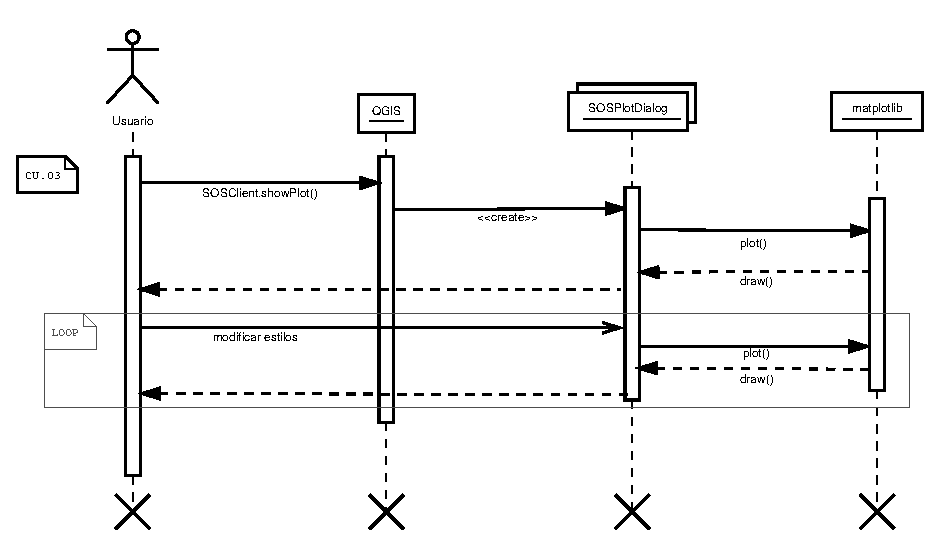
\includegraphics[width=\textwidth]{images/seq3.eps}
 \caption{Diagrama de secuencia para o caso de uso \ref{uc:CU.03}}
 \label{fig:diaSeq3}
\end{figure}

Para cubrir a funcionalidade requirida polo caso de uso \ref{uc:CU.04} existe o \emph{plugin} \emph{TimeManager} para QGIS, polo que o que representa o diagrama \ref{fig:diaSeq4} é o procedemento para que a capa xerada coas observacións sexa controlada polo \emph{TimeManager}.
\begin{figure}
 \centering
 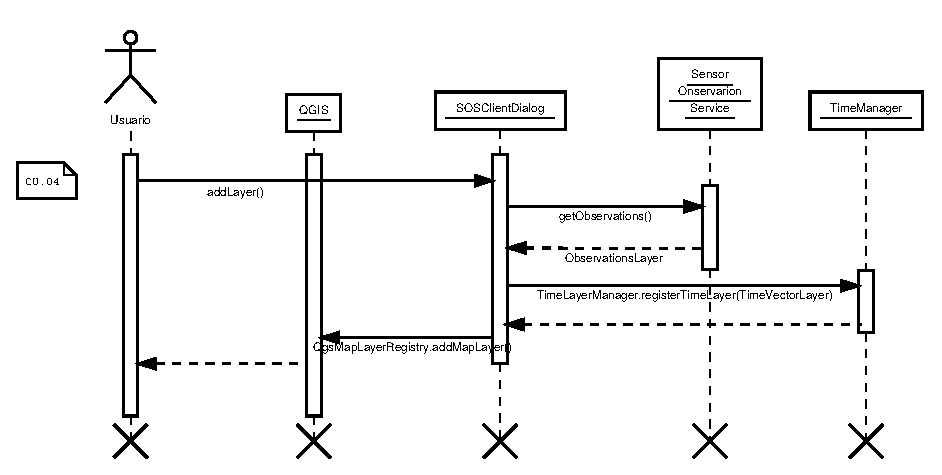
\includegraphics[width=\textwidth]{images/seq4.eps}
 \caption{Diagrama de secuencia para o caso de uso \ref{uc:CU.04}}
 \label{fig:diaSeq4}
\end{figure}